% This must be in the first 5 lines to tell arXiv to use pdfLaTeX, which is strongly recommended.
\pdfoutput=1
% In particular, the hyperref package requires pdfLaTeX in order to break URLs across lines.

\documentclass[11pt]{article}

\usepackage[review]{acl}

% Standard package includes
\usepackage{times}
\usepackage{latexsym}
\usepackage{amsmath}
\usepackage{graphicx}
\usepackage{booktabs}

% For proper rendering and hyphenation of words containing Latin characters (including in bib files)
\usepackage[T1]{fontenc}
% For Vietnamese characters
% \usepackage[T5]{fontenc}
% See https://www.latex-project.org/help/documentation/encguide.pdf for other character sets

% This assumes your files are encoded as UTF8
\usepackage[utf8]{inputenc}

% This is not strictly necessary, and may be commented out.
% However, it will improve the layout of the manuscript,
% and will typically save some space.
\usepackage{microtype}

% This is also not strictly necessary, and may be commented out.
% However, it will improve the aesthetics of text in
% the typewriter font.
\usepackage{inconsolata}


% If the title and author information does not fit in the area allocated, uncomment the following
%
%\setlength\titlebox{<dim>}
%
% and set <dim> to something 5cm or larger.

\title{CSC401 Homework Assignment \#2\\Analysis}

\author{Firstname Lastname \\
  Student number: \texttt{123456} \\
  UTORid: \texttt{abcdef} \\
  \texttt{name@mail.utoronto.ca}}

\begin{document}
\maketitle

\section{Training Results}

\subsection{Training Loop Printout}
Place your training loop printout in this section. The numbers shown are for illustration purposes only and the loss and BLEU values presented are fabricated.

\paragraph{Model with Pre-layer Normalization}
\begin{small}
\begin{verbatim}
[Device:cuda] Epoch 1 Training ====
Forward Step:      1/  2171 | Accumulation Step:   0 | Loss:   97.88 | Learning Rate: 8.5e-80
Forward Step:    201/  2171 | Accumulation Step:  10 | Loss:   32.59 | Learning Rate: 9.4e-23
...
\end{verbatim}
\end{small}

\vspace{2em}

Alternatively, you can depict the WandB graphs as shown in figure \ref{fig:train_bleu_wo_attention} \& \ref{fig:train_loss_wo_attention}. The numbers shown are for illustration purposes only and the loss and BLEU values presented are fabricated. You should expect very different outcomes.  We recommend exporting your charts as {\tt .png} files following this tutorial: \url{https://wandb.ai/site/articles/export-data-from-wb}.

\begin{figure}[hbt!]
\centering
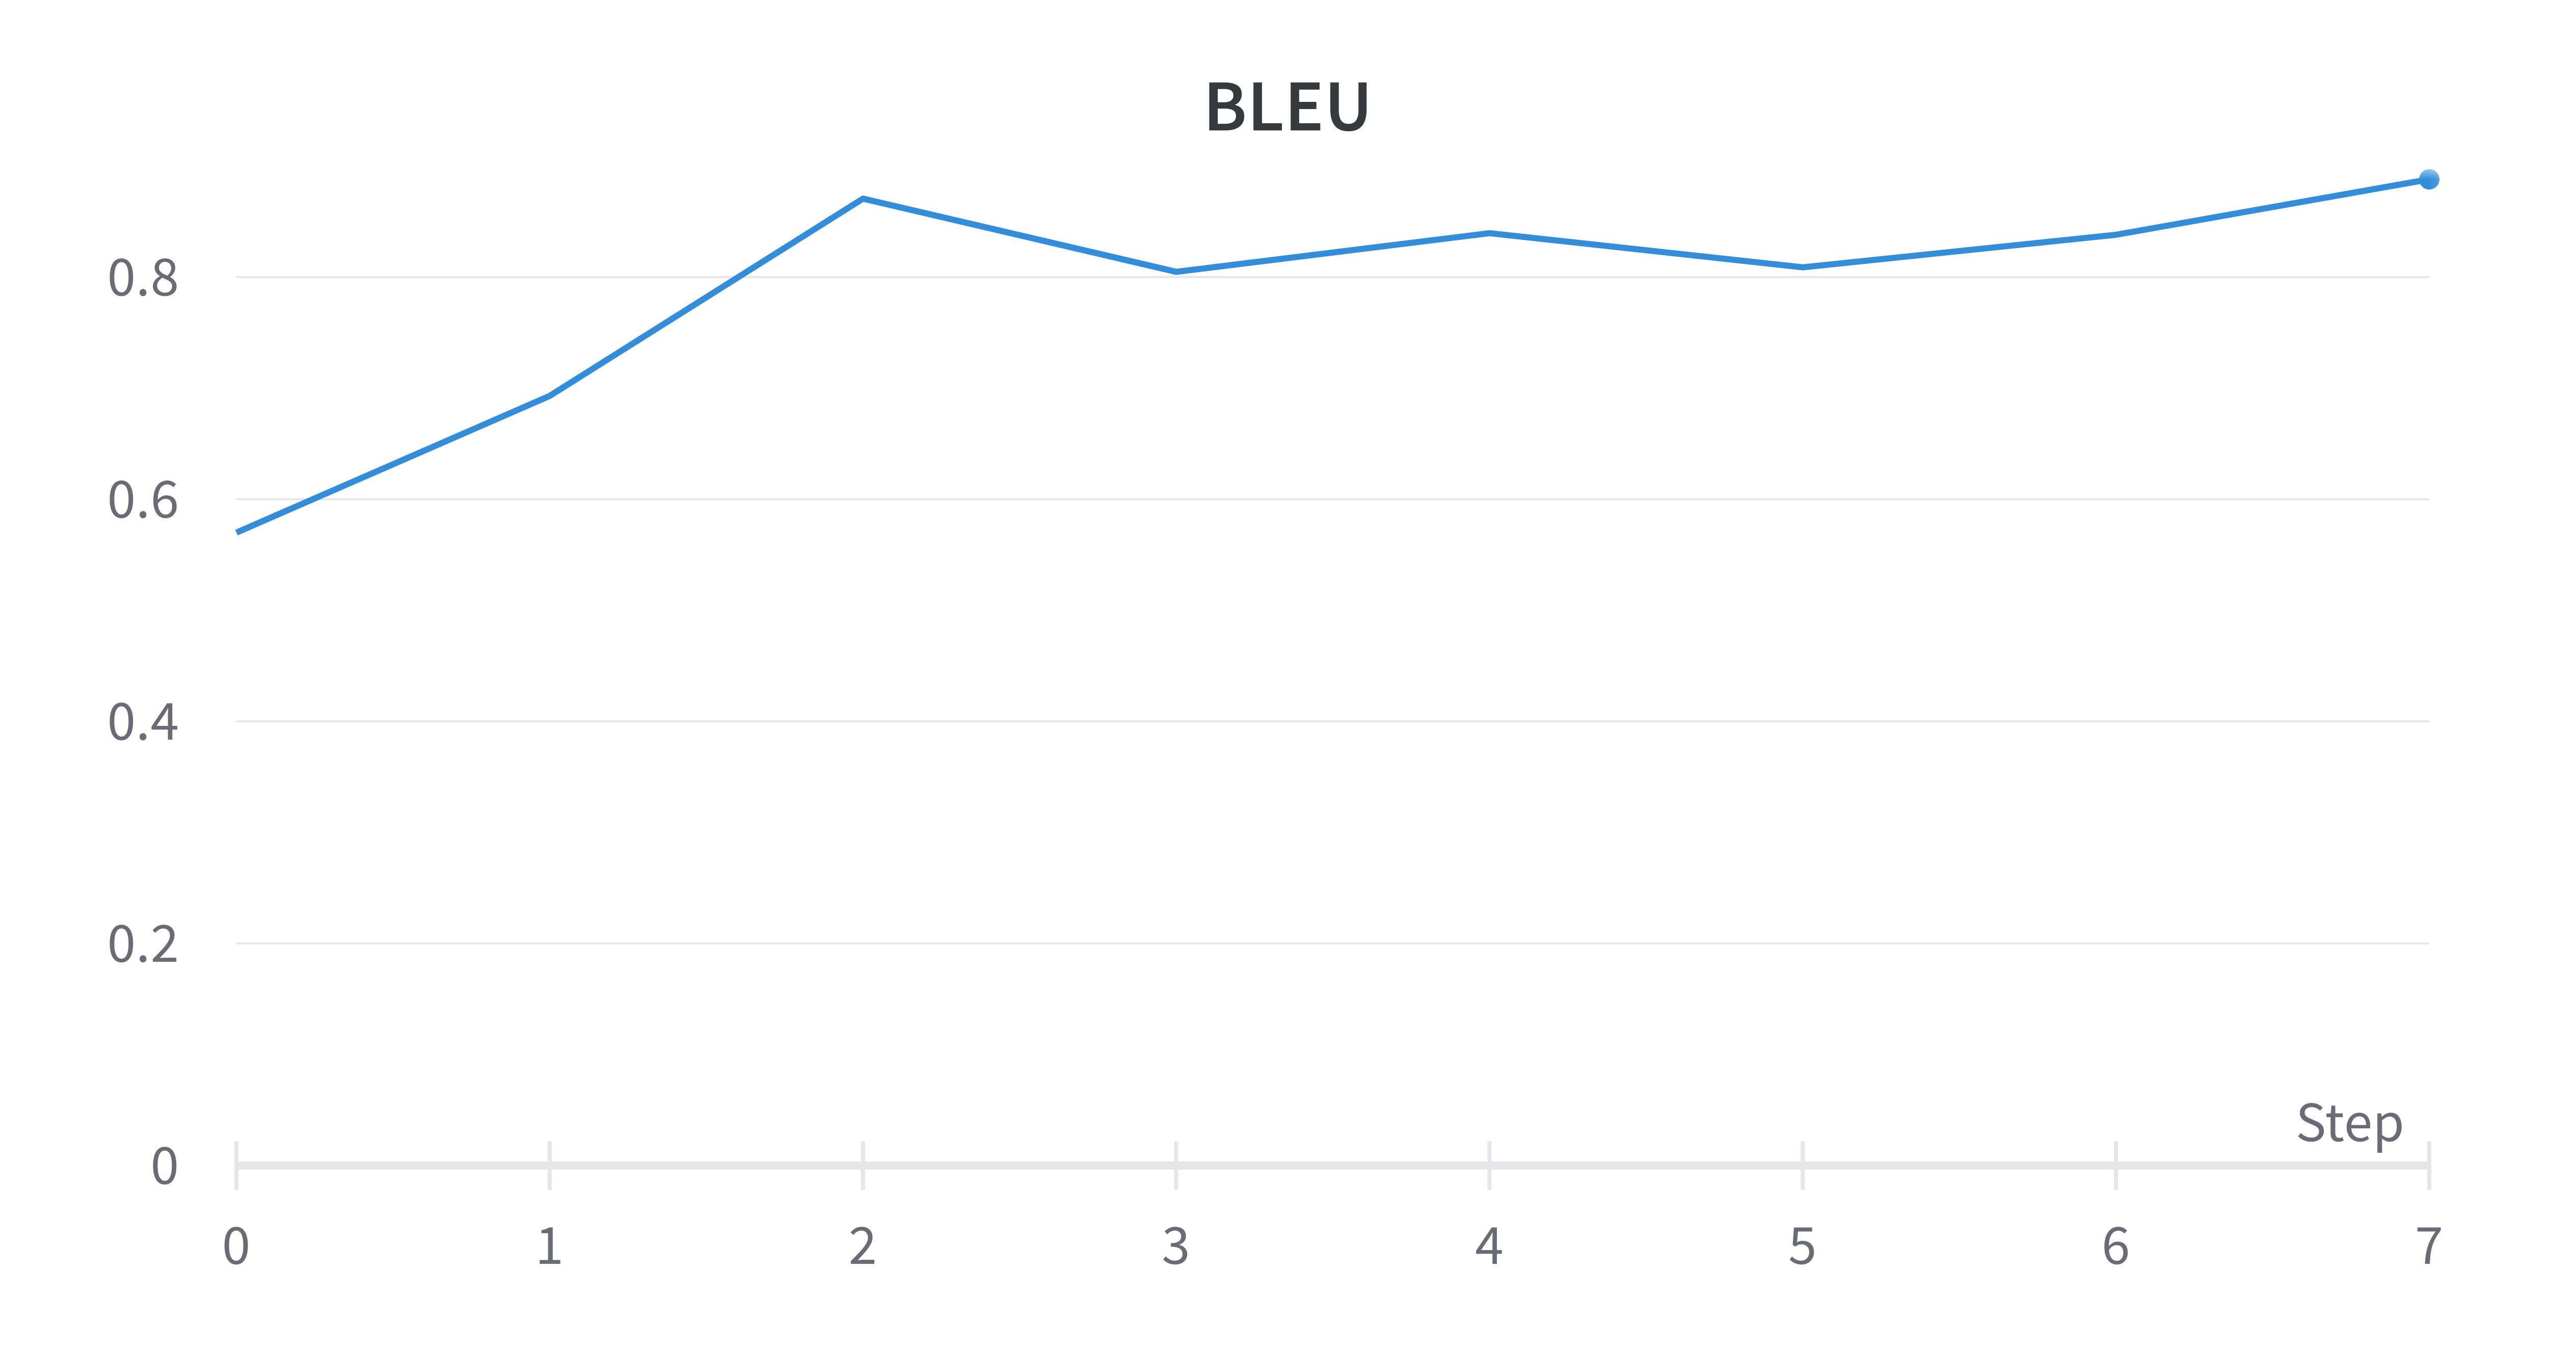
\includegraphics[width=0.65\linewidth]{./wandb_bleu.png}
\caption{Wandb Training BLEU Score for Model with Pre-layer Normalization}
\label{fig:train_bleu_wo_attention}
\end{figure}

\begin{figure}[hbt!]
\centering
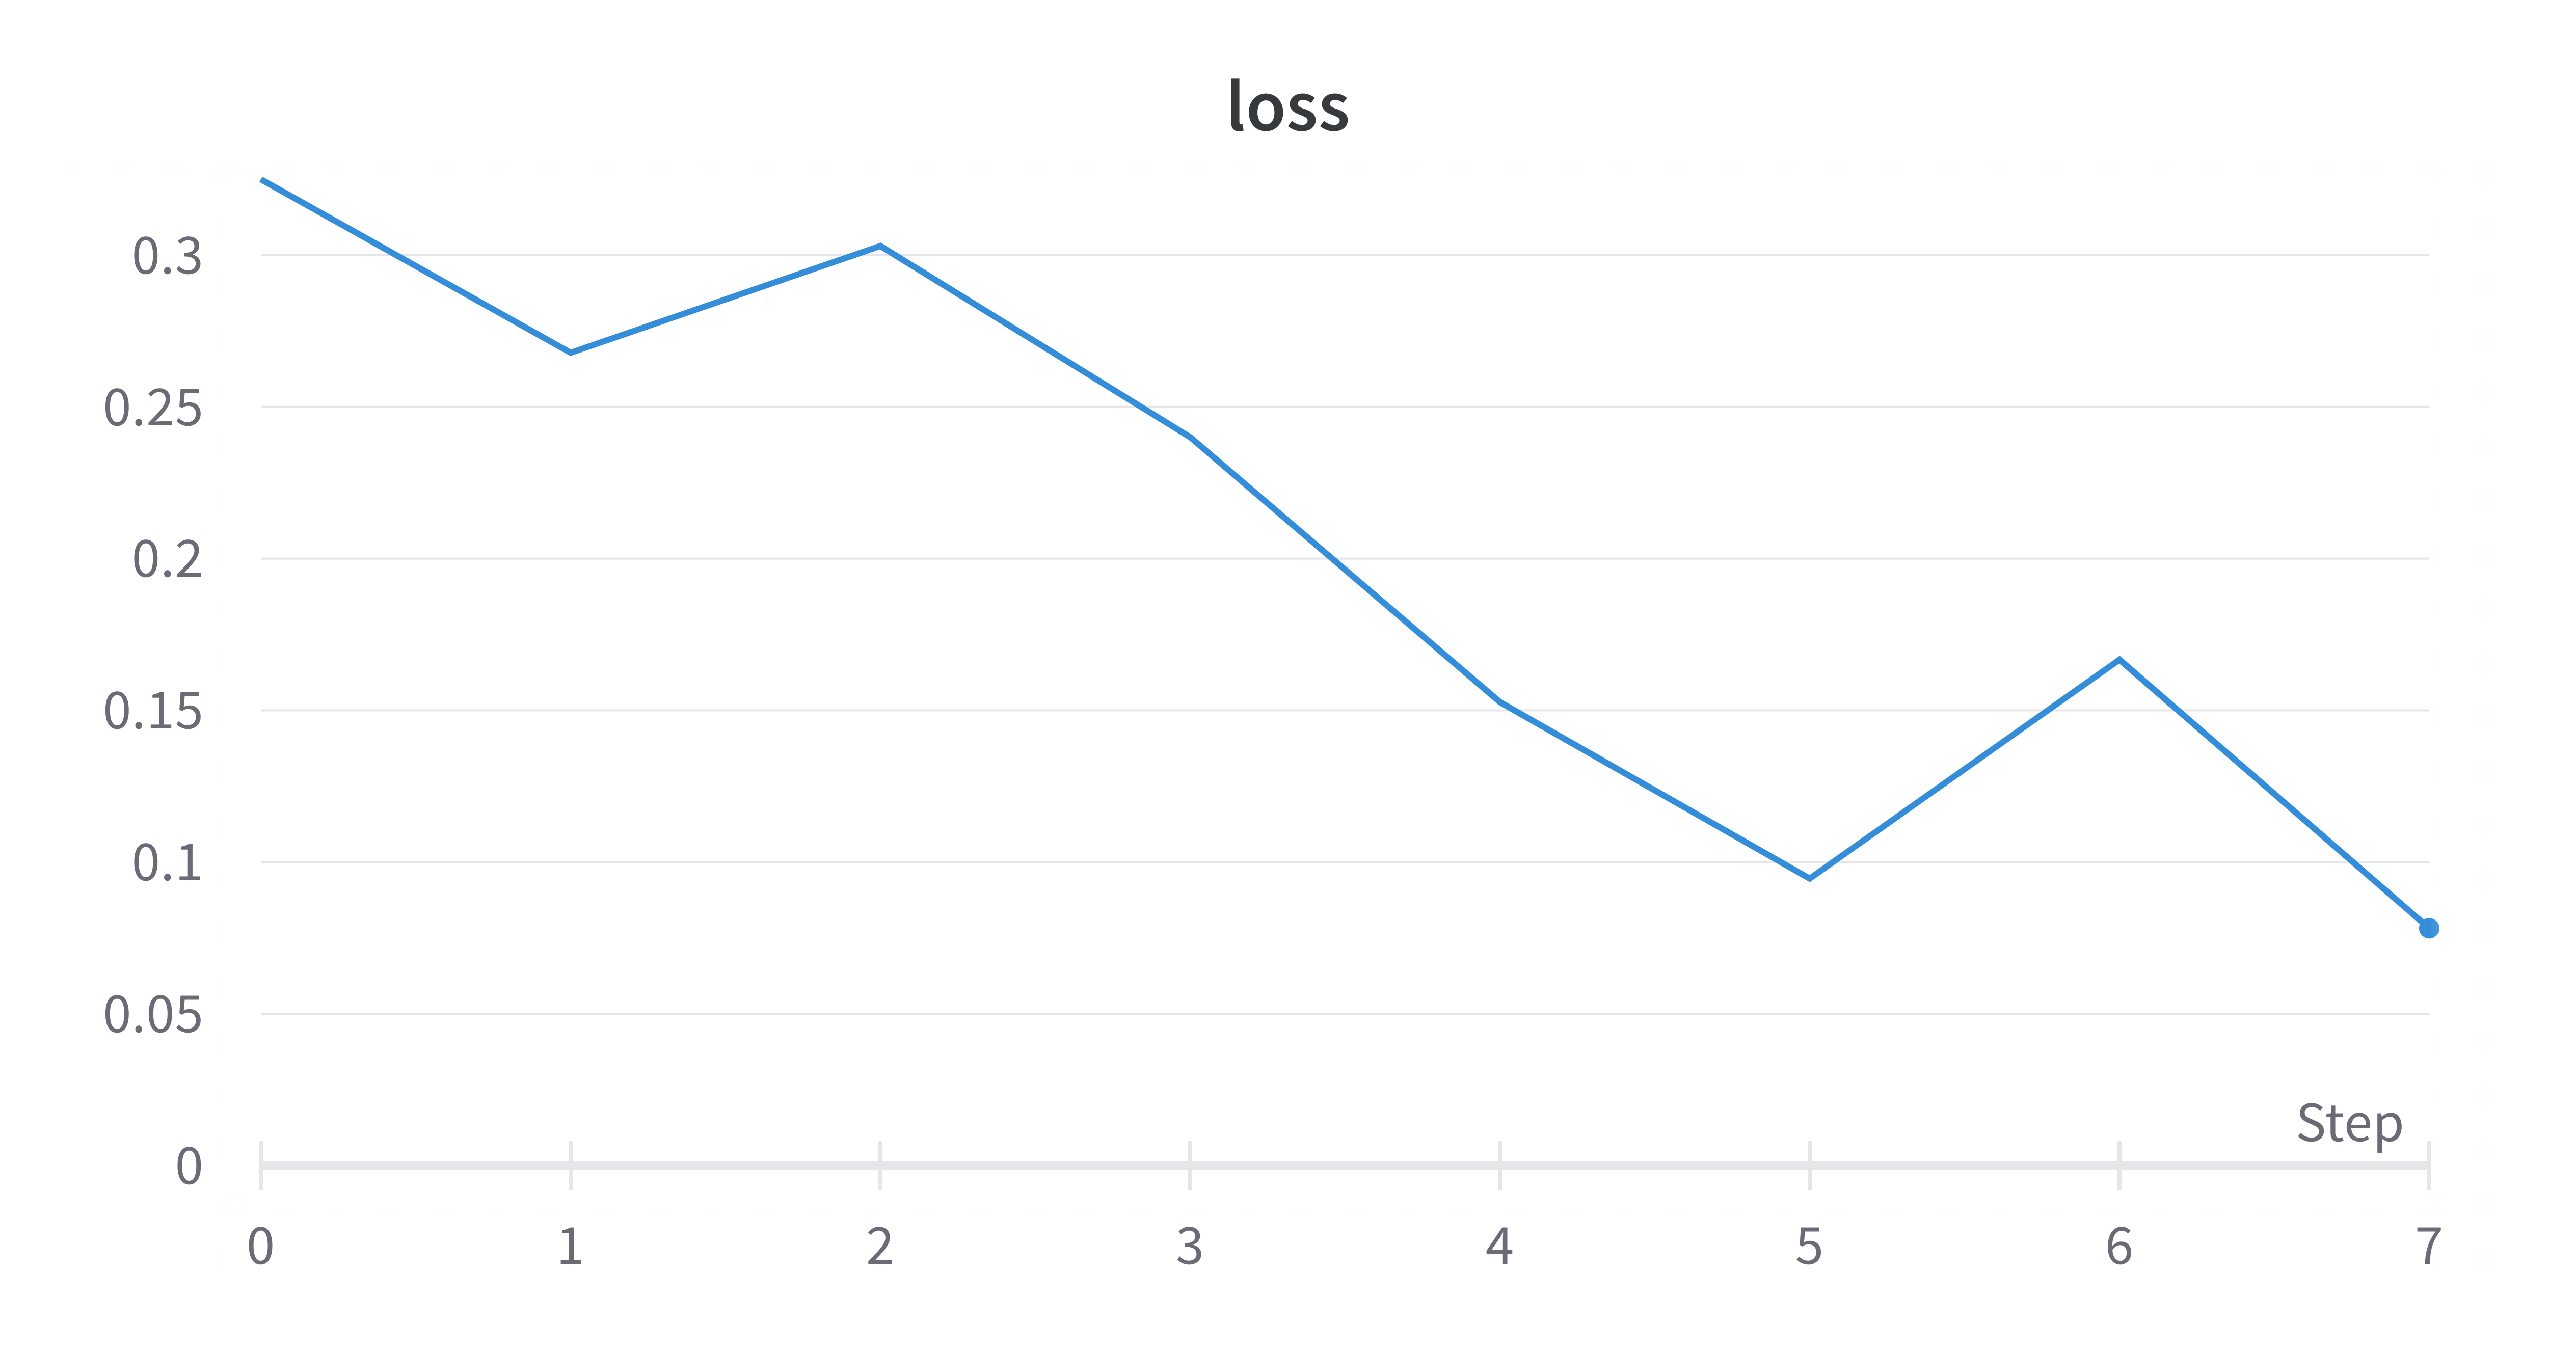
\includegraphics[width=0.65\linewidth]{./wandb_loss.png}
\caption{Wandb Training Loss for Model with Pre-layer Normalization}
\label{fig:train_loss_wo_attention}
\end{figure}

\paragraph{Model with Post-layer Normalization}


\subsection{Test Set BLEU Score}
This section lists the test set BLEU score reported on the test set for each model in table \ref{tab:bleu}.
\begin{table}[h]
\centering
\begin{tabular}{lcc} \toprule
Model                          & BLEU-4 &  BLEU-3 \\ \midrule
Model Pre-layer Normalization  & 0.0    \\
Model Post-layer Normalization & 0.0    \\
\bottomrule
\end{tabular}
\caption{The BLEU score reported on the test set for each model.}
\label{tab:bleu}
\end{table}

\section{Translation Analysis}

\subsection{Translations}

List all of your translations in this section.

\subsection{Discussion}
{\it In this section, write a brief discussion on your findings. Describe the quality of
those sentences. How's your model compared with Google Translate or ChatGPT?}

\end{document}
